%%%%% Magnetisches Feld %%%%%
%%  %%


%Some sample text to be displayed above the first subsection

%\subsection{Prinzip}

%Ein Zyklotron besteht aus Zwei hohlen, halbzylindrischen und Duanden an denen eine Spannung mit unterschiedlichem Vorzeichen anliegt, und darüber bzw. darunter liegende Magneten, die ein homogenes Magnetfeld erzeugen. Zudem gibt es einen Einlass und einen Auslass für Teilchen.

%\begin{wrapfigure}{r}{0.4\textwidth} \label{Zyklo}
%
%	\vspace{-10pt}
%	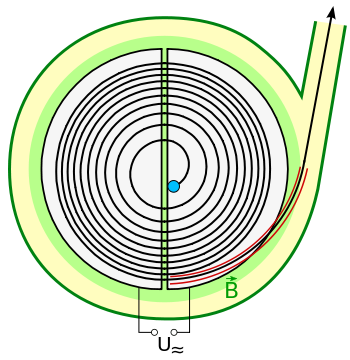
\includegraphics[width=0.35\textwidth]{Zyklotron_Prinzipskizze02.png}
%	\vspace{-13pt}
%	\caption{Prinzipskizze eines Zyklotrons}
%	\vspace{-5pt}	
%	
%\end{wrapfigure}

%\subsubsection{Anwendung}

% Some Formula:

%\begin{equation}
%	x= \frac{y \cdot 13 \pi z}
%			{\cos \alpha}
%\end{equation}

%%%%%%%%%%%%%%%%%%%%%%%
% Eigentlicher Beginn %
%%%%%%%%%%%%%%%%%%%%%%%


\subsection{Feldlinien}

Wie schon beim elektrischen Feld wird hier ein Feldlinienmodell genutzt um die Eigenschaften wie Ausrichtung (Polung) und Stärke darzustellen. 

Magnetische Felder haben 2 Pole, nicht negativ oder positiv, wie beim elektrischen Feld, sondern sie werden Nord- und Südpol genannt. Ungleichnamige Pole ziehen sich an, gleichnamige stoßen sich ab. Im Feldlinienmodell zeigen die Pfeile immer zum Südpol.

Charakteristische Bilder von Feldlinien sowie Erklärungen zu diesen finden sich in \referenz{sec:feldlinienbilder}


\subsection{Magnetische Flussdichte}

Auch beim magnetischen Feld gibt die Dichte eine Größe zur Bestimmung der Stärke des Feldes an. Diese heißt aber nicht Feldstärke sondern \glqq magnetische Flussdichte \grqq{} (Formelzeichen $B$, Einheit \glqq Telsa\grqq : $T=\frac{kg}{As^2}=\frac{Vs}{m^2}$) (die magnetische Feldstärke gibt es auch, bezeichnet aber etwas anderes!). Diese ist also äquivalent zur Feldstärke des elektrischen Feldes und ordnet über die Lorentzkraft jedem bewegten, geladenen Teilchen eine Kraft zu (Siehe \referenz{subsec:BLorentzDefinition}).


\subsection{Homogenes Feld}

Ein homogenes Magnetfeld hat die Eigenschaft, dass die Flussdichte in jedem Punkt gleich ist, was das Berechnen erheblich einfacher macht. (Vergleiche: \referenz{subsec:EFeldHomogen}) Homogene Felder treten z.B. im inneren von Spulen oder zwischen den Schenkeln eines Hufeisenmagneten auf. Mehr dazu in \referenz{sec:feldlinienbilder}.

















